\documentclass[leqno]{article}
% Shared QBT/Soln pack preamble for resources.danieljsmith.org.
\usepackage{graphicx}
\usepackage{dsfont}
\usepackage{mathtools}
\usepackage{amssymb}
\usepackage{amsmath}
\usepackage{amsthm}
\usepackage{float}
\usepackage{ragged2e}
\usepackage{tensor}
\usepackage{fancyhdr}
\usepackage{empheq}
\usepackage[most]{tcolorbox}
\usepackage{enumitem}
\usepackage{dirtytalk}
\usepackage{marginnote}
\usepackage{microtype}
\usepackage[
  a4paper,
  left=0.8in,
  right=1in,
  top=1in,
  bottom=0.5in,
  headheight=14pt,
  headsep=0.4in
]{geometry}
\setlength{\parindent}{0cm}

% TikZ / PGFPlots
\usepackage{pgfplots}
\pgfplotsset{compat=1.18}
\usepgfplotslibrary{fillbetween, polar}
\usetikzlibrary{calc, positioning}
\usetikzlibrary{angles, quotes}
\usetikzlibrary{arrows.meta}
\usetikzlibrary{decorations.pathreplacing, decorations.markings}
\usetikzlibrary{patterns}
\usetikzlibrary{intersections}

% Links and contents
\usepackage[colorlinks=true,linkcolor=black,citecolor=magenta,urlcolor=black]{hyperref}%
\urlstyle{same}

% Pack macros
\RenewDocumentCommand{\marks}{o m}{%
  \IfValueTF{#1}%
    {\marginnote{\raggedright\textbf{[#2]}}[#1]}%
    {\marginnote{\raggedright\textbf{[#2]}}}%
}

\newcommand{\vspacerule}[2]{%
  \par\vspace*{#1}%
  \noindent\hrulefill\par
  \vspace*{#2}%
}

\definecolor{scarlet}{RGB}{205, 40, 75}

% Worked-solution box, adapted from the TMUA worked-solutions box. A white breakable box with a left scarlet rule and no surrounding
% frame or tint. A part that breaks fills the rest of its page, so the rule
% runs to the bottom margin; the unbroken or last part ends in a short
% horizontal foot rule so a solution visibly stops. Unlike the TMUA box there
% is no answer label and no extra \parskip: these solutions mix \\ line breaks
% with blank lines, so paragraph skips would make the spacing uneven. The box
% does not grow to the left, so the rule sits at the text edge; growing to the
% right keeps the usable line width close to the old tcolorbox Solution box.
\newtcolorbox{djsSolution}{%
  enhanced, breakable, frame hidden, sharp corners, colback=white,
  height fixed for=first and middle, height fill,
  extras unbroken and last={natural height},
  borderline west={2.2pt}{0pt}{scarlet},
  left=11pt, right=0pt, top=5pt, bottom=13pt,
  before skip=13pt, after skip=4pt,
  grow to right by=10mm,
  overlay unbroken and last={%
    \fill[scarlet] (frame.south west)
      rectangle ([xshift=3.5cm, yshift=2.2pt]frame.south west);},
  before upper={{\color{scarlet}\bfseries Solution}\par\vspace{4pt}}}

% Optional smaller figure inside a solution box. \scalebox shrinks node text
% with the drawing. Not applied to existing figures.
\newcommand{\SolnFigureScale}{0.85}
\newsavebox{\djsSolnFigureBox}
\newenvironment{djsSolutionFigure}
  {\par\vspace{4pt}\begin{center}\begin{lrbox}{\djsSolnFigureBox}}
  {\end{lrbox}\scalebox{\SolnFigureScale}{\usebox{\djsSolnFigureBox}}%
   \end{center}\vspace{2pt}\par}

\newcommand{\cxl}[2]{%
  \tikz[baseline=(X.base)]{%
    \node[inner sep=0pt, outer sep=0pt, text=#1] (X) {$#2$};
    \draw[#1, line width=0.4pt] (X.south west)--(X.north east);
  }%
}

% Page-style hook run at the contents page and each question's opening page.
% A no-op for QBT packs; \djsSolnHeader points it at the fancy header.
\newcommand{\djsQuestionPageStyle}{}

\newcommand{\questionitem}{%
  \djsQuestionPageStyle
  \item\phantomsection
  \addcontentsline{toc}{section}{Question \number\value{enumi}}%
}

\renewcommand{\contentsname}{Questions}

\newcommand{\djsPackHeader}[1]{%
  \pagestyle{fancy}%
  \fancyhead{}%
  \fancyfoot{}%
  \renewcommand{\headrulewidth}{0.9pt}%
  \lhead{#1}%
  \chead{}%
  \rhead{\href{https://danieljsmith.org}{danieljsmith.org}}%
}

\newcommand{\djsQbtHeader}[1]{%
  \djsPackHeader{#1}%
}

% Solutions packs show the header only on the contents page and each
% question's opening page, so it never appears part-way through a solution.
% \thispagestyle marks the next page shipped out, which is the question's
% page because every solution question starts after a \newpage.
\newcommand{\djsSolnHeader}[1]{%
  \djsPackHeader{\textit{Solutions} - #1}%
  \pagestyle{empty}%
  \renewcommand{\djsQuestionPageStyle}{\thispagestyle{fancy}}%
}

\newcommand{\djsFrontMatter}{%
  \djsQuestionPageStyle
  \vspace*{20pt}%
  \tableofcontents
  \newpage
}


\djsSolnHeader{Power and Driving Force}

\begin{document}
\djsFrontMatter
\begin{enumerate}[
  label=\textbf{\arabic*.},
  leftmargin=*,
  topsep=0pt,
  partopsep=0pt,
  parsep=0pt
]

% ---- Question 1 ----
\questionitem
% [Source: _QBT___Solns___Power_and_Driving_Force_, Q1]

A delivery van of mass $2000\,\mathrm{kg}$ is travelling up a straight road inclined at angle $\alpha$ to the horizontal, where $\sin\alpha=0.05$. \\

The van's engine can produce power at a maximum rate of $64\,\mathrm{kW}$. \\

The total resistance force due to friction and air resistance is modelled as $(200+kv)\,\mathrm{N}$, where $v\,\mathrm{m\,s^{-1}}$ is the speed of the van and $k$ is a constant. \\

The greatest possible constant speed of the van up the hill is $20\,\mathrm{m\,s^{-1}}$. \\

Find the maximum possible acceleration of the van when it is travelling uphill at $16\,\mathrm{m\,s^{-1}}$. \\

Fully justify your answer. \marks{7} \\

\vspace*{10pt}

\begin{tcolorbox}[colback=white, colframe=scarlet, title={\textbf{Solution}}, breakable, grow to left by=6mm, grow to right by=10mm]
For motion up the slope, the forces acting down the slope are the resistance and the component of weight.

The component of weight down the slope is
\[
2000g\sin\alpha = 2000 \times 9.8 \times \frac{1}{20} = 980\,\mathrm{N}
\]

If the engine provides driving force $F$ when the speed is $v$, then
\[
P = Fv
\]
so
\[
F = \frac{P}{v}
\]

At the greatest possible constant speed, $v=20\,\mathrm{m\,s^{-1}}$. Since the speed is constant, the acceleration is $0$, so the resultant force is $0$. Also, the engine must be working at its maximum power; otherwise a larger power would give a larger driving force, so the van could travel at a higher constant speed, which contradicts the statement that $20\,\mathrm{m\,s^{-1}}$ is the greatest possible constant speed.

So the driving force at $20\,\mathrm{m\,s^{-1}}$ is
\[
F = \frac{64000}{20} = 3200\,\mathrm{N}
\]

The resistance at this speed is
\[
200 + 20k
\]

Balancing forces along the slope gives
\begin{align*}
3200 &= (200+20k) + 980 \\
3200 &= 1180 + 20k \\
20k &= 2020 \\
k &= 101
\end{align*}

Now consider the van when it is travelling at $16\,\mathrm{m\,s^{-1}}$.

To get the maximum possible acceleration, we need the maximum possible resultant force up the slope. At this speed, the weight component and the resistance are fixed, so this happens when the engine again uses its maximum power.

Hence the maximum possible driving force is
\[
F = \frac{64000}{16} = 4000\,\mathrm{N}
\]

The resistance force at $16\,\mathrm{m\,s^{-1}}$ is
\[
200 + kv = 200 + 101(16) = 1816\,\mathrm{N}
\]

So the resultant force up the slope is
\[
4000 - 1816 - 980 = 1204\,\mathrm{N}
\]

Using Newton's second law,
\[
1204 = 2000a
\]
so
\[
a = \frac{1204}{2000} = 0.602\,\mathrm{m\,s^{-2}}
\]

Hence the maximum possible acceleration of the van is $0.602\,\mathrm{m\,s^{-2}}$.
\end{tcolorbox}


\newpage

% ---- Question 2 ----
\questionitem
% [Source: _QBT___Solns___Power_and_Driving_Force_, Q2]

A delivery van has mass $1300\,\mathrm{kg}$ and travels on a straight horizontal road. \\

In a simple model, the van experiences a constant rolling resistance of $600$ newtons and an additional air-resistance force whose magnitude is proportional to the speed of the van. \\

During a test, the van moves at a steady speed of $15\,\mathrm{m\,s^{-1}}$ when the engine provides a driving force of $1200$ newtons. \\

In this model, the engine can deliver a constant maximum power. The greatest speed the van can attain on this road is $30\,\mathrm{m\,s^{-1}}$. \\

\begin{enumerate}[label=\textbf{(\alph*)}]
  \item Show that the maximum power of the engine is $54\,000\,\mathrm{W}$ \marks{2} \\
  \item Find the maximum acceleration of the van when it is travelling at $20\,\mathrm{m\,s^{-1}}$ \marks{3} \\
  \item Find the maximum acceleration of the van when it is travelling at $4\,\mathrm{m\,s^{-1}}$ \marks{1} \\
  \item Comment on the validity of the model in the context of your answers to parts (b) and (c). \marks{2} \\
\end{enumerate}

\vspace*{10pt}

\begin{tcolorbox}[colback=white, colframe=scarlet, title={\textbf{Solution}}, breakable, grow to left by=6mm, grow to right by=10mm]
\begin{enumerate}[label=\textbf{(\alph*)}, start=1]
  \item Let the air-resistance force be \(kv\), where \(v\) is the speed.

At a steady speed of \(15\,\mathrm{m\,s^{-1}}\), the acceleration is zero, so the driving force equals the total resistance:
\[
1200 = 600 + 15k
\]
Hence
\[
15k = 600 \quad \Rightarrow \quad k=40
\]
So the total resistance at speed \(v\) is
\[
600+40v
\]

At the greatest speed \(30\,\mathrm{m\,s^{-1}}\), the van is again moving steadily, so
\[
\text{driving force} = 600+40(30)=1800\,\mathrm{N}
\]
Using
\[
\text{power} = \text{force} \times \text{speed}
\]
we get
\[
P = 1800 \times 30 = 54000\,\mathrm{W}
\]
So the maximum power of the engine is \(54000\,\mathrm{W}\).

  \item At \(20\,\mathrm{m\,s^{-1}}\), using the maximum power found in part (a),
\[
P=Fv \quad \Rightarrow \quad F=\frac{P}{v}=\frac{54000}{20}=2700\,\mathrm{N}
\]
So the maximum driving force is \(2700\,\mathrm{N}\).

The resistance at \(20\,\mathrm{m\,s^{-1}}\) is
\[
600+40(20)=1400\,\mathrm{N}
\]
Therefore the resultant forward force is
\[
2700-1400=1300\,\mathrm{N}
\]
Using \(F=ma\),
\[
1300 = 1300a
\]
so
\[
a=1\,\mathrm{m\,s^{-2}}
\]
Thus the maximum acceleration is \(1\,\mathrm{m\,s^{-2}}\).

  \item At \(4\,\mathrm{m\,s^{-1}}\), the maximum driving force is
\[
F=\frac{54000}{4}=13500\,\mathrm{N}
\]
The resistance is
\[
600+40(4)=760\,\mathrm{N}
\]
So the resultant force is
\[
13500-760=12740\,\mathrm{N}
\]
Hence
\[
a=\frac{12740}{1300}=9.8\,\mathrm{m\,s^{-2}}
\]
Thus the maximum acceleration is \(9.8\,\mathrm{m\,s^{-2}}\).

  \item The answer in part (b), \(1\,\mathrm{m\,s^{-2}}\), is reasonable for a delivery van.

However, the answer in part (c), \(9.8\,\mathrm{m\,s^{-2}}\), is unrealistically large for a van. This suggests the model is not valid at low speeds.

The reason is that with constant power,
\[
F=\frac{P}{v}
\]
so as \(v\) gets smaller, the model predicts a much larger driving force. In fact, as \(v \to 0\), the force would become extremely large, which is not realistic.

So the constant-power model is reasonable at higher speeds, but not at low speeds.
\end{enumerate}
\end{tcolorbox}


\newpage

% ---- Question 3 ----
\questionitem
% [Source: _QBT___Solns___Power_and_Driving_Force_, Q3]

A maintenance vehicle of mass $1000\,\mathrm{kg}$ moves on a straight slope inclined at an angle $\theta$ to the horizontal, where $\sin\theta=0.08$. When the motor is switched off, the vehicle coasts down the slope and reaches a limiting speed of $14\,\mathrm{m\,s^{-1}}$. The resistance to motion is proportional to the square of the speed. The motor is then switched on and works at a constant power $P\,\mathrm{W}$, allowing the vehicle to travel up the same slope with a limiting speed of $10\,\mathrm{m\,s^{-1}}$. \\

Find the value of $P$ and determine the resistance to motion when the vehicle is travelling at $12\,\mathrm{m\,s^{-1}}$ \marks{10} \\

\vspace*{10pt}

\begin{tcolorbox}[colback=white, colframe=scarlet, title={\textbf{Solution}}, breakable, grow to left by=6mm, grow to right by=10mm]
Let the resistance to motion at speed \(v\) be
\[
R=kv^2
\]
where \(k\) is a constant.

At a limiting speed, the acceleration is zero, so the resultant force along the slope is zero.

When the motor is switched off, the vehicle moves \emph{down} the slope with limiting speed \(14\,\mathrm{m\,s^{-1}}\). The component of the weight down the slope is
\[
mg\sin\theta = 1000\times 9.8\times 0.08 = 784\,\mathrm{N}
\]
At limiting speed, this is balanced by the resistance, so
\[
k(14)^2=784
\]
Hence
\[
196k=784
\]
so
\[
k=4
\]
Therefore the resistance is
\[
R=4v^2
\]

Now the motor is switched on and the vehicle travels \emph{up} the slope with limiting speed \(10\,\mathrm{m\,s^{-1}}\).

If the driving force is \(F\), then using
\[
\text{power} = \text{force} \times \text{speed}
\]
we have
\[
P=Fv
\]
So when \(v=10\),
\[
F=\frac{P}{10}
\]

The forces opposing the upward motion are:
\[
\text{weight component} = 784\,\mathrm{N}
\]
and
\[
\text{resistance} = 4(10)^2=400\,\mathrm{N}
\]
Since the speed is limiting, resultant force is zero, so
\[
\frac{P}{10}=784+400
\]
Hence
\[
\frac{P}{10}=1184
\]
and therefore
\[
P=11840\,\mathrm{W}
\]
That is
\[
P=11.84\,\mathrm{kW}
\]

When the vehicle is travelling at \(12\,\mathrm{m\,s^{-1}}\), the resistance is
\[
R=4(12)^2=4\times 144=576\,\mathrm{N}
\]

Therefore, the motor power is \(11840\,\mathrm{W}\) \((11.84\,\mathrm{kW})\), and the resistance to motion at \(12\,\mathrm{m\,s^{-1}}\) is \(576\,\mathrm{N}\).
\end{tcolorbox}


\newpage

% ---- Question 4 ----
\questionitem
% [Source: _QBT___Solns___Power_and_Driving_Force_, Q4]

\begin{figure}[H]
    \centering
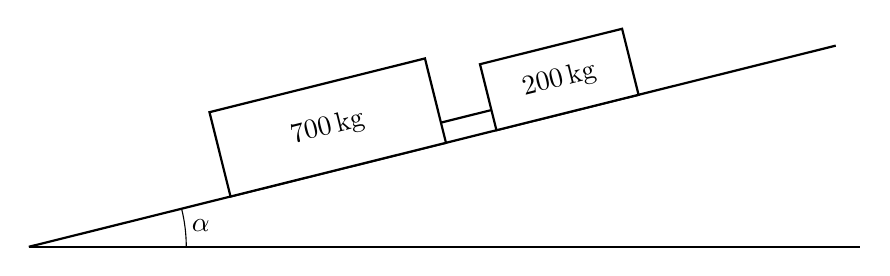
\begin{tikzpicture}[scale=1.2]
\def\ang{14}
\def\planelen{8.8}
\def\carx{2.2}
\def\clen{2.35}
\def\cheight{0.92}
\def\tlen{1.55}
\def\theight{0.72}
\def\gap{0.55}
\def\hitchh{0.22}
\pgfmathsetmacro{\trailx}{\carx+\clen+\gap}

\coordinate (A) at (0,0);
\coordinate (B) at (\ang:\planelen);
\coordinate (H) at (\planelen,0);
\coordinate (Cpos) at (\ang:\carx);
\coordinate (Tpos) at (\ang:\trailx);

\draw[thick] (A) -- (B);
\draw[thick] (A) -- (H);
\pic["$\alpha$", draw, angle radius=20mm, angle eccentricity=1.1] {angle=H--A--B};

\begin{scope}[shift={(Cpos)}, rotate=\ang]
  \coordinate (CarTow) at (\clen,\hitchh);
  \draw[thick, fill=white] (0,0) rectangle (\clen,\cheight);
  \node[rotate=\ang] at ({0.5*\clen},{0.5*\cheight}) {$700\,\mathrm{kg}$};
\end{scope}

\begin{scope}[shift={(Tpos)}, rotate=\ang]
  \coordinate (TraTow) at (0,\hitchh);
  \draw[thick, fill=white] (0,0) rectangle (\tlen,\theight);
  \node[rotate=\ang] at ({0.5*\tlen},{0.5*\theight}) {$200\,\mathrm{kg}$};
\end{scope}

\draw[thick] (CarTow) -- (TraTow);
\end{tikzpicture}
\end{figure}


A car of mass $700\,\mathrm{kg}$ is descending a straight road which is inclined at an angle $\alpha$ to the horizontal, where $\sin\alpha=\tfrac{1}{10}$. The car is connected to a trailer of mass $200\,\mathrm{kg}$ by a light rigid towbar which is parallel to the road, as shown in the diagram. \\

The resistance to the motion of the car is modelled as a constant force of magnitude $240\,\mathrm{N}$. 

The resistance to the motion of the trailer is modelled as a constant force of magnitude $90\,\mathrm{N}$. \\

The brakes of the car dissipate energy at a constant rate of $9\,\mathrm{kW}$. \\

Find the force in the towbar at the instant when the speed of the car is $12\,\mathrm{m\,s^{-1}}$, stating whether the towbar is in tension or compression. \marks{8} \\

\vspace*{10pt}

\begin{tcolorbox}[colback=white, colframe=scarlet, title={\textbf{Solution}}, breakable, grow to left by=6mm, grow to right by=10mm]
Since the car is moving \emph{down} the slope, the resistances and the braking force all act \emph{up} the slope.

The brakes dissipate energy at a rate of $9\,\mathrm{kW}=9000\,\mathrm{W}$.
Using
\[
P=Fv
\]
at the instant when $v=12\,\mathrm{m\,s^{-1}}$, the braking force is
\[
F=\frac{P}{v}=\frac{9000}{12}=750\,\mathrm{N}
\]
This force acts up the slope.

Take up the slope as positive.

For the car and trailer together, the total mass is
\[
700+200=900\,\mathrm{kg}
\]
The component of their total weight down the slope is
\[
900g\sin\alpha=900g\left(\frac{1}{10}\right)=90g
\]
So, resolving along the slope for the whole system,
\begin{align*}
240+90+750-90g &= 900a \\
1080-90g &= 900a
\end{align*}
With $g=9.8$,
\[
1080-90(9.8)=900a
\]
\[
1080-882=900a
\]
\[
198=900a
\]
\[
a=\frac{198}{900}=0.22\,\mathrm{m\,s^{-2}}
\]
So the acceleration is $0.22\,\mathrm{m\,s^{-2}}$ up the slope.

Now consider the trailer alone.
Let $T$ be the force in the towbar on the trailer, taken positive up the slope.

For the trailer, resolving along the slope,
\begin{align*}
T+90-200g\sin\alpha &= 200a \\
T+90-200g\left(\frac{1}{10}\right) &= 200(0.22) \\
T+90-20g &= 44
\end{align*}
Substitute $g=9.8$:
\begin{align*}
T+90-196 &= 44 \\
T-106 &= 44 \\
T &= 150
\end{align*}
Hence the force in the towbar has magnitude
\[
150\,\mathrm{N}
\]

This force on the trailer is \emph{up} the slope. If the towbar were in tension, it would pull the trailer \emph{down} the slope towards the car. So the towbar must be in \textbf{compression}.

Therefore, the force in the towbar is $150\,\mathrm{N}$, in compression.
\end{tcolorbox}


\newpage

% ---- Question 5 ----
\questionitem
% [Source: _QBT___Solns___Power_and_Driving_Force_, Q5]

An airport tug of mass $1800\,\mathrm{kg}$ has an engine that can deliver a maximum power of $72\,\mathrm{kW}$. \\

In an initial model of the motion of the tug, the total resistance to motion is assumed to be constant. \\

\begin{enumerate}[label=(\roman*)]
  \item Given that the greatest steady speed of the tug on a straight horizontal runway is $18\,\mathrm{m\,s^{-1}}$, find the magnitude of the resistance force. \marks{2} \\
  \item The tug is connected to a small aircraft of mass $2200\,\mathrm{kg}$ by a light rigid horizontal tow bar. The greatest steady speed of the tug and aircraft on the runway is now $12\,\mathrm{m\,s^{-1}}$. The resistance to motion of the aircraft may also be assumed constant. \\

  Find the magnitude of the resistance force on the aircraft. \marks{2} \\
  \item The tug and aircraft again travel along the runway. At one instant their speed is $10\,\mathrm{m\,s^{-1}}$ and their acceleration is $0.25\,\mathrm{m\,s^{-2}}$. \\

  \begin{enumerate}[label=(\alph*)]
    \item Find the power of the engine of the tug at this instant. \marks{4}
    \item Find the magnitude of the force in the tow bar at this instant. \marks{2}\\
  \end{enumerate}
  \item In a refined model of the motion of the tug and aircraft, the resistance to motion of each is assumed to be zero until they reach a speed of $6\,\mathrm{m\,s^{-1}}$. When the speed is $6\,\mathrm{m\,s^{-1}}$ or above, the same constant resistance forces as in the first model are assumed to apply to each. \\

  The tug and aircraft start from rest on the runway and accelerate, using maximum power. \\

  Without carrying out any further calculations,
  \begin{enumerate}[label=(\alph*)]
    \item explain whether the time taken to attain a speed of $10\,\mathrm{m\,s^{-1}}$ would be predicted to be lower, the same or higher using the refined model compared with the original model. \marks{2}
    \item explain whether the greatest steady speed of the system would be predicted to be lower, the same or higher using the refined model compared with the original model. \marks{2}
  \end{enumerate}
\end{enumerate}

\vspace*{10pt}

\begin{tcolorbox}[colback=white, colframe=scarlet, title={\textbf{Solution}}, breakable, grow to left by=6mm, grow to right by=10mm]
\begin{enumerate}[label=\textbf{(\roman*)}, start=1]
  \item At greatest steady speed on a horizontal runway, the acceleration is zero, so the driving force equals the resistance.

  Using
  \[
  P = Fv
  \]
  gives
  \[
  R_{\text{tug}} = \frac{72000}{18} = 4000\,\mathrm{N}
  \]
  Hence the resistance force on the tug is \(4000\,\mathrm{N}\).

  \item For the tug and aircraft together, at the greatest steady speed the total driving force equals the total resistance.

  So
  \[
  R_{\text{total}} = \frac{72000}{12} = 6000\,\mathrm{N}
  \]
  Therefore the resistance on the aircraft is
  \[
  R_{\text{aircraft}} = 6000 - 4000 = 2000\,\mathrm{N}
  \]
  Hence the resistance force on the aircraft is \(2000\,\mathrm{N}\).

  \item
  \begin{enumerate}[label=\textbf{(\alph*)}, start=1]
    \item The total mass is
    \[
    1800 + 2200 = 4000\,\mathrm{kg}
    \]
    So the resultant force is
    \[
    ma = 4000 \times 0.25 = 1000\,\mathrm{N}
    \]
    The total resistance is
    \[
    4000 + 2000 = 6000\,\mathrm{N}
    \]
    Hence the driving force of the engine is
    \[
    1000 + 6000 = 7000\,\mathrm{N}
    \]
    Therefore the power at this instant is
    \[
    P = Fv = 7000 \times 10 = 70000\,\mathrm{W} = 70\,\mathrm{kW}
    \]
    So the power of the engine is \(70\,\mathrm{kW}\).

    \item Let the force in the tow bar be \(T\).

    Considering the aircraft alone,
    \[
    T - 2000 = 2200 \times 0.25
    \]
    so
    \begin{align*}
    T - 2000 &= 550 \\
    T &= 2550
    \end{align*}
    So the magnitude of the force in the tow bar is \(2550\,\mathrm{N}\).
  \end{enumerate}

  \item
  \begin{enumerate}[label=\textbf{(\alph*)}, start=1]
    \item The time would be \emph{lower}.

    In the refined model, there is no resistance until the speed reaches \(6\,\mathrm{m\,s^{-1}}\). So below \(6\,\mathrm{m\,s^{-1}}\), the resultant force is greater than in the original model, and hence the acceleration is greater.

    From \(6\) to \(10\,\mathrm{m\,s^{-1}}\), both models are the same. Therefore the refined model predicts a smaller time to reach \(10\,\mathrm{m\,s^{-1}}\).

    \item The greatest steady speed would be \emph{the same}.

    From part (ii), the greatest steady speed of the system is \(12\,\mathrm{m\,s^{-1}}\), which is above \(6\,\mathrm{m\,s^{-1}}\). So at that speed, both models use the same resistance forces. Since the maximum engine power is also the same, the predicted greatest steady speed is unchanged.
  \end{enumerate}
\end{enumerate}
\end{tcolorbox}


\newpage

% ---- Question 6 ----
\questionitem
% [Source: _QBT___Solns___Power_and_Driving_Force_, Q6]

A snowmobile of mass $800\,\mathrm{kg}$ tows a rescue sledge of mass $200\,\mathrm{kg}$ up a straight slope that is inclined at angle $\theta$ to the horizontal. The sledge is attached to the snowmobile by a light inextensible rope. The resistance to the motion of the snowmobile from non-gravitational forces is modelled as a constant force of magnitude $216\,\mathrm{N}$. The resistance to the motion of the sledge from non-gravitational forces is modelled as a constant force of magnitude $294\,\mathrm{N}$. \\

When the engine of the snowmobile is working at a constant rate of $12\,\mathrm{kW}$, the snowmobile and the sledge move up the slope with constant speed $12\,\mathrm{m\,s^{-1}}$. \\

\begin{enumerate}[label=\textbf{(\alph*)}]
  \item Find the value of $\sin\theta$. \marks{4} \\
  \item Later, at the instant when the snowmobile and the sledge are travelling down the slope with speed $14\,\mathrm{m\,s^{-1}}$, the rope snaps. When the rope snaps the sledge is at the point $A$. The sledge continues to travel down the slope before coming to instantaneous rest at the point $B$. The resistance to the motion of the sledge from non-gravitational forces is again modelled as a constant force of magnitude $294\,\mathrm{N}$. \\

  Use the work-energy principle, and your answer to part (a), to find the distance $AB$. \marks{5} \\
\end{enumerate}

\vspace*{10pt}

\begin{tcolorbox}[colback=white, colframe=scarlet, title={\textbf{Solution}}, breakable, grow to left by=6mm, grow to right by=10mm]
\begin{enumerate}[label=\textbf{(\alph*)}, start=1]
  \item Take the snowmobile and sledge together as one system, so the rope tension is internal.

  Let the driving force of the engine be \(D\). Since power \(P = Dv\),
  \begin{align*}
  D &= \frac{P}{v} \\
    &= \frac{12000}{12} \\
    &= 1000\ \mathrm{N}
  \end{align*}

  The total mass is
  \[
  800 + 200 = 1000\ \mathrm{kg}
  \]

  So the component of the total weight down the slope is \(1000g\sin\theta\), and the total resistance is
  \[
  216 + 294 = 510\ \mathrm{N}
  \]

  As the speed is constant, the resultant force along the slope is zero. Hence
  \[
  1000 = 1000g\sin\theta + 510
  \]

  So
  \begin{align*}
  1000g\sin\theta &= 490 \\
  9800\sin\theta &= 490 \\
  \sin\theta &= 0.05
  \end{align*}

  Therefore,
  \[
  \sin\theta = 0.05
  \]

  \item Let \(AB = s\) m.

  Use the work-energy principle
  \[
  KE_0 + GPE_0 + \sum W_{\text{other}} = KE_1 + GPE_1
  \]

  Take state 0 at \(A\) and state 1 at \(B\).

  For the sledge,
  \begin{align*}
  KE_0 &= \tfrac12 \times 200 \times 14^2 = 19600\ \mathrm{J} \\
  KE_1 &= 0
  \end{align*}

  The resistance acts up the slope while the sledge moves down the slope, so the work done by resistance is
  \[
  \sum W_{\text{other}} = -294s
  \]

  The vertical drop from \(A\) to \(B\) is \(s\sin\theta\), so
  \[
  GPE_0 - GPE_1 = 200gs\sin\theta
  \]

  Substituting into the work-energy equation,
  \[
  19600 + 200gs\sin\theta - 294s = 0
  \]

  Using \(\sin\theta = 0.05\),
  \begin{align*}
  19600 + 200(9.8)(0.05)s - 294s &= 0 \\
  19600 + 98s - 294s &= 0 \\
  19600 - 196s &= 0 \\
  s &= 100
  \end{align*}

  Therefore,
  \[
  AB = 100\ \mathrm{m}
  \]
\end{enumerate}
\end{tcolorbox}


\newpage

% ---- Question 7 ----
\questionitem
% [Source: _QBT___Solns___Power_and_Driving_Force_, Q7]

A lorry of mass $3200\,\mathrm{kg}$ tows a trailer of mass $1800\,\mathrm{kg}$ down a line of greatest slope of a straight road inclined at an angle $\theta$ to the horizontal, where $\sin\theta=0.06$. \\

The power developed by the lorry's engine is constant. The resistances to motion of the lorry and the trailer are constant and equal to $800\,\mathrm{N}$ and $500\,\mathrm{N}$ respectively. When the lorry passes through a point $A$ on the road, the speed of the combination is $14\,\mathrm{m\,s^{-1}}$ and its acceleration is $1.2\,\mathrm{m\,s^{-2}}$. \\

\begin{enumerate}[label=\textbf{(\alph*)}]
  \item Calculate the power developed by the engine. \marks{5} \\
  \item The lorry later passes through a point $B$ on the road with speed $22\,\mathrm{m\,s^{-1}}$. The time taken for the lorry to travel from $A$ to $B$ is $7.93\,\mathrm{s}$. \\

  Find the distance $AB$. \marks{5} \\
\end{enumerate}

\vspace*{10pt}

\begin{tcolorbox}[colback=white, colframe=scarlet, title={\textbf{Solution}}, breakable, grow to left by=6mm, grow to right by=10mm]
\begin{enumerate}[label=\textbf{(\alph*)}, start=1]
  \item The total mass of the lorry and trailer is
  \[
  3200+1800=5000\,\mathrm{kg}
  \]

  Take the direction down the slope as positive.

  Let the driving force of the engine when the speed is $14\,\mathrm{m\,s^{-1}}$ be $F$ N.
  Since power $=$ force $\times$ speed,
  \[
  P=Fv \qquad \Rightarrow \qquad F=\frac{P}{14}
  \]

  Resolving forces down the slope for the lorry-trailer combination,
  \[
  F+5000g\sin\theta-(800+500)=5000(1.2)
  \]

  Substitute $g=9.8$ and $\sin\theta=0.06$.
  \[
  F+5000(9.8)(0.06)-1300=6000
  \]
  \[
  F+2940-1300=6000
  \]
  \[
  F=4360\,\mathrm{N}
  \]

  Hence
  \[
  P=Fv=4360\times 14=61040\,\mathrm{W}
  \]

  So the power developed by the engine is
  \[
  6.104\times 10^4\,\mathrm{W}=61.0\,\mathrm{kW}
  \]

  \item Let the distance $AB$ be $s$ m.

  Use the work-energy principle:
  \[
  KE_A+GPE_A+\sum W_{\text{other}}=KE_B+GPE_B
  \]

  Here:
  \begin{itemize}
    \item the work done by the engine from $A$ to $B$ is $Pt$,
    \item the work done against resistance is $-(800+500)s=-1300s$,
    \item moving down the slope through distance $s$ reduces the GPE by
    \[
    5000g(s\sin\theta)=5000\times 9.8\times 0.06\,s=2940s
    \]
    so $GPE_B=GPE_A-2940s$.
  \end{itemize}

  Therefore
  \begin{align*}
  \frac12(5000)(14^2)+GPE_A+Pt-1300s
  &=\frac12(5000)(22^2)+GPE_A-2940s
  \end{align*}

  With $P=61040\,\mathrm{W}$ and $t=7.93\,\mathrm{s}$,
  \begin{align*}
  \frac12(5000)(14^2)+61040(7.93)-1300s
  &=\frac12(5000)(22^2)-2940s
  \\
  61040(7.93)+1640s
  &=\frac12(5000)(22^2-14^2)
  \\
  61040(7.93)+1640s
  &=720000
  \end{align*}

  So
  \[
  s=\frac{720000-61040(7.93)}{1640}=143.874\ldots
  \]

  Hence
  \[
  AB\approx 144\,\mathrm{m}
  \]
\end{enumerate}
\end{tcolorbox}


\newpage

% ---- Question 8 ----
\questionitem
% [Source: _QBT___Solns___Power_and_Driving_Force_, Q8]

A lorry of mass $2500\,\mathrm{kg}$ travels up a straight road inclined at an angle $\alpha$ to the horizontal, where $\tan\alpha=\dfrac{7}{24}$. \\

The engine of the lorry supplies a constant power of $P\,\mathrm{W}$. The total resistance to motion is a constant force of magnitude $R\,\mathrm{N}$. \\

When the lorry is moving at $12\,\mathrm{m\,s^{-1}}$, its acceleration is $2.4\,\mathrm{m\,s^{-2}}$. When it is moving at $18\,\mathrm{m\,s^{-1}}$, its acceleration is $0.4\,\mathrm{m\,s^{-2}}$. \\

Find the value of $P$ and the value of $R$ \marks{8} \\

\vspace*{10pt}

\begin{tcolorbox}[colback=white, colframe=scarlet, title={\textbf{Solution}}, breakable, grow to left by=6mm, grow to right by=10mm]
Take motion up the slope as positive.

Since \(\tan\alpha=\dfrac{7}{24}\), we use the \(7\!:\!24\!:\!25\) triangle, so
\[
\sin\alpha=\frac{7}{25}
\]
Hence the component of the lorry's weight acting down the slope is
\[
mg\sin\alpha=2500\times 9.8\times \frac{7}{25}=6860\text{ N}
\]

If the lorry is moving with speed \(v\), then
\[
\text{driving force} = \frac{\text{power}}{\text{speed}}=\frac{P}{v}
\]
So, resolving along the slope,
\[
\frac{P}{v}-R-6860=2500a
\]

Using \(v=12\) and \(a=2.4\),
\begin{align*}
\frac{P}{12}-R-6860&=2500(2.4)\\
\frac{P}{12}-R-6860&=6000\\
\frac{P}{12}-R&=12860
\end{align*}

Using \(v=18\) and \(a=0.4\),
\begin{align*}
\frac{P}{18}-R-6860&=2500(0.4)\\
\frac{P}{18}-R-6860&=1000\\
\frac{P}{18}-R&=7860
\end{align*}

Now subtract the second equation from the first:
\begin{align*}
\left(\frac{P}{12}-R\right)-\left(\frac{P}{18}-R\right)&=12860-7860\\
\frac{P}{12}-\frac{P}{18}&=5000\\
P\left(\frac{1}{12}-\frac{1}{18}\right)&=5000\\
P\left(\frac{1}{36}\right)&=5000
\end{align*}
So
\[
P=180000\text{ W}
\]

Substitute into \(\dfrac{P}{18}-R=7860\):
\begin{align*}
\frac{180000}{18}-R&=7860\\
10000-R&=7860\\
R&=2140
\end{align*}

Therefore,
\[
P=1.80\times 10^5\text{ W},\qquad R=2140\text{ N}
\]
\end{tcolorbox}


\newpage

% ---- Question 9 ----
\questionitem
% [Source: _QBT___Solns___Power_and_Driving_Force_, Q9]

A van of mass $1000\,\mathrm{kg}$ is driven up a straight road inclined at an angle $\alpha$ to the horizontal, where $\sin\alpha=\dfrac{1}{20}$. The engine is working at a constant rate of $12\,\mathrm{kW}$ and the van moves at a constant speed of $15\,\mathrm{m\,s^{-1}}$. \\

\begin{enumerate}[label=\textbf{(\alph*)}]
  \item Find the resistance to the motion of the van. \marks{4} \\
  \item The van now tows a trailer of mass $600\,\mathrm{kg}$ up the same road using a tow rope parallel to the line of motion. The resistance to the motion of the van is the same as in part (a), and the resistance to the motion of the trailer is a constant force of magnitude $106\,\mathrm{N}$. \\

  The engine is still working at a constant rate of $12\,\mathrm{kW}$. \\

  The tow rope is modelled as light and inextensible. \\

  Using the model, find the tension in the tow rope at the instant when the speed of the van is $7.5\,\mathrm{m\,s^{-1}}$. \marks{5} \\
\end{enumerate}

\vspace*{10pt}

\begin{tcolorbox}[colback=white, colframe=scarlet, title={\textbf{Solution}}, breakable, grow to left by=6mm, grow to right by=10mm]
\begin{enumerate}[label=\textbf{(\alph*)}, start=1]
  \item Let the resistance to the motion of the van be \(R\,\mathrm{N}\).

  The engine power is \(12\,\mathrm{kW}=12000\,\mathrm{W}\). Using
  \[
  P=Fv
  \]
  gives the driving force:
  \[
  12000=F\times 15
  \]
  \[
  F=800\,\mathrm{N}
  \]

  The van moves at constant speed, so its acceleration is zero. Hence the resultant force along the slope is zero.

  Taking up the slope as positive,
  \[
  800=R+1000\times 9.8\times \frac{1}{20}
  \]
  \[
  800=R+490
  \]
  \[
  R=310
  \]

  So the resistance to the motion of the van is \(310\,\mathrm{N}\).

  \item When the speed is \(7.5\,\mathrm{m\,s^{-1}}\), the engine is still working at \(12000\,\mathrm{W}\), so the driving force is
  \[
  F=\frac{P}{v}=\frac{12000}{7.5}=1600\,\mathrm{N}
  \]

  First consider the van and trailer together as one system.

  Their total mass is
  \[
  1000+600=1600\,\mathrm{kg}
  \]

  The total force opposing the motion up the slope is
  \[
  310+106+1600\times 9.8\times \frac{1}{20}
  \]
  \[
  =310+106+784=1200\,\mathrm{N}
  \]

  So the resultant force up the slope is
  \[
  1600-1200=400\,\mathrm{N}
  \]

  Hence the acceleration is
  \[
  a=\frac{400}{1600}=0.25\,\mathrm{m\,s^{-2}}
  \]

  The tow rope is light and inextensible, so the trailer has the same acceleration.

  Now consider the trailer alone. Taking up the slope as positive,
  \[
  T-106-600\times 9.8\times \frac{1}{20}=600\times 0.25
  \]
  \[
  T-106-294=150
  \]
  \[
  T=550
  \]

  So the tension in the tow rope is \(550\,\mathrm{N}\).
\end{enumerate}
\end{tcolorbox}


\newpage

% ---- Question 10 ----
\questionitem
% [Source: _QBT___Solns___Power_and_Driving_Force_, Q10]

A lorry of mass $2400\,\mathrm{kg}$ is towing a trailer of mass $600\,\mathrm{kg}$ up a straight road inclined at an angle $\theta$ to the horizontal, where $\sin\theta=\dfrac{1}{49}$. \\

When the lorry and trailer move at speed $v\,\mathrm{m\,s^{-1}}$, the total resistance to motion has magnitude $(300+60v)\,\mathrm{N}$. \\

The greatest constant speed that the lorry and trailer can maintain on this hill is $15\,\mathrm{m\,s^{-1}}$. \\

Find the maximum power output of the lorry's engine. \\

Fully justify your answer. \marks{5} \\

\vspace*{10pt}

\begin{tcolorbox}[colback=white, colframe=scarlet, title={\textbf{Solution}}, breakable, grow to left by=6mm, grow to right by=10mm]
For the lorry and trailer together, the total mass is
\[
2400+600=3000\text{ kg}
\]

The component of the total weight acting down the slope is
\[
3000g\sin\theta=3000\times 9.8\times \frac{1}{49}=600\text{ N}
\]

When the speed is \(v\,\mathrm{m\,s^{-1}}\), the given resistance to motion is \((300+60v)\,\mathrm{N}\), so the total opposing force is
\[
600+(300+60v)=900+60v\text{ N}
\]

At constant speed, the resultant force is zero, so the engine's driving force must be \(900+60v\) N.

Using
\[
\text{power}=\text{force}\times\text{speed}
\]
the power needed to maintain speed \(v\) is
\[
P(v)=v(900+60v)=900v+60v^2
\]

Now justify why we can use \(v=15\). Differentiate:
\[
\frac{\mathrm{d}P}{\mathrm{d}v}=900+120v
\]

For all relevant speeds \(v\ge 0\),
\[
900+120v>0
\]

So \(P(v)\) increases as \(v\) increases. Therefore the greatest constant speed that can be maintained, \(15\,\mathrm{m\,s^{-1}}\), must occur when the engine is producing its maximum power.

Hence
\[
P_{\max}=P(15)=15(900+60\times 15)=15(1800)=27000\text{ W}
\]

So the maximum power output of the lorry's engine is \(27000\text{ W}=27\text{ kW}\).
\end{tcolorbox}


\newpage

% ---- Question 11 ----
\questionitem
% [Source: _QBT___Solns___Power_and_Driving_Force_, Q11]

A maintenance train has mass $10\,000\,\mathrm{kg}$ and the maximum power of its engine is $200\,\mathrm{kW}$. In a model of the train's motion, it is assumed that while the train is moving the total resistance to motion is constant. \\

On a straight horizontal track, the greatest constant speed that the train can maintain when the engine is working at maximum power is $20\,\mathrm{m\,s^{-1}}$. \\

\begin{enumerate}[label=\textbf{(\alph*)}]
  \item Find the resistance to motion. \marks{2} \\
  \item While the train is still on horizontal track, the engine is delivering $60\,\mathrm{kW}$ when the speed of the train is $8\,\mathrm{m\,s^{-1}}$. \\
  Find the acceleration of the train at this instant. \marks{2} \\
  \item The train then climbs a straight track inclined at an angle $\theta$ above the horizontal. When the engine is working at maximum power, the greatest constant speed that the train can maintain is $10\,\mathrm{m\,s^{-1}}$. \\
  Determine the value of $\theta$. \marks{3} \\
\end{enumerate}

\vspace*{10pt}

\begin{tcolorbox}[colback=white, colframe=scarlet, title={\textbf{Solution}}, breakable, grow to left by=6mm, grow to right by=10mm]
\begin{enumerate}[label=\textbf{(\alph*)}, start=1]
  \item At the greatest constant speed on horizontal track, the train has zero acceleration, so the resultant force is zero. Hence the tractive force equals the resistance, say $R$.

Using $P=Fv$,
\[
200\,000 = R \times 20
\]
so
\[
R = 10\,000\ \mathrm{N}
\]

So the resistance to motion is $10\,000\ \mathrm{N}$.

  \item When the power is $60\,\mathrm{kW}$ and the speed is $8\,\mathrm{m\,s^{-1}}$, the tractive force is
\[
F=\frac{P}{v}=\frac{60\,000}{8}=7500\ \mathrm{N}
\]

So the resultant forward force is
\[
7500-10\,000=-2500\ \mathrm{N}
\]

Using $F=ma$,
\[
a=\frac{-2500}{10\,000}=-0.25\ \mathrm{m\,s^{-2}}
\]

So the acceleration is $-0.25\ \mathrm{m\,s^{-2}}$.

  \item On the incline, at the greatest constant speed $10\,\mathrm{m\,s^{-1}}$, the train again has zero acceleration, so the tractive force balances the resistance and the component of weight down the slope.

At maximum power,
\[
F=\frac{P}{v}=\frac{200\,000}{10}=20\,000\ \mathrm{N}
\]

The forces opposing the motion are
\[
R + mg\sin\theta = 10\,000 + 10\,000\times 9.8\sin\theta
\]

So
\[
20\,000 = 10\,000 + 10\,000\times 9.8\sin\theta
\]
\[
10\,000 = 98\,000\sin\theta
\]
\[
\sin\theta = \frac{10\,000}{98\,000}=\frac{5}{49}
\]

Therefore
\[
\theta=\sin^{-1}\left(\frac{5}{49}\right)\approx 5.86^\circ
\]

So $\theta=\sin^{-1}\!\left(\frac{5}{49}\right)\approx 5.86^\circ$.
\end{enumerate}
\end{tcolorbox}


\newpage

% ---- Question 12 ----
\questionitem
% [Source: _QBT___Solns___Power_and_Driving_Force_, Q12]

A rail maintenance vehicle of mass $2000\,\mathrm{kg}$ travels in a straight line along a horizontal section of track at a constant speed of $20\,\mathrm{m\,s^{-1}}$. \\

The resistance to the motion of the vehicle is modelled as a constant force of magnitude $2000\,\mathrm{N}$. \\

The engine is working at a constant rate of $P\,\mathrm{kW}$. \\

Using the model, \\

\begin{enumerate}[label=\textbf{(\alph*)}]
  \item find the value of $P$. \marks{3} \\
\end{enumerate}

The vehicle now travels up a straight section of track which is inclined to the horizontal at an angle $\alpha$, where $\sin \alpha = \dfrac{1}{20}$. \\

In a refined model, the resistance to the motion of the vehicle from non-gravitational forces is modelled as a force of magnitude $(220 + 2v^2)\,\mathrm{N}$, where $v\,\mathrm{m\,s^{-1}}$ is the speed. \\

At the instant when the engine is working at the same constant rate as in part (a) and the vehicle is moving up the track at $10\,\mathrm{m\,s^{-1}}$, the acceleration of the vehicle is $a\,\mathrm{m\,s^{-2}}$. \\

Using the refined model, \\

\begin{enumerate}[label=\textbf{(\alph*)}, resume]
  \item find the value of $a$. \marks{4} \\
\end{enumerate}

Later, when the engine is again working at this constant rate, the vehicle is moving up the track at a constant speed $U\,\mathrm{m\,s^{-1}}$. \\

Using the refined model, \\

\begin{enumerate}[label=\textbf{(\alph*)}, resume]
  \item find the value of $U$. \marks{5} \\
\end{enumerate}

\vspace*{10pt}

\begin{tcolorbox}[colback=white, colframe=scarlet, title={\textbf{Solution}}, breakable, grow to left by=6mm, grow to right by=10mm]
\begin{enumerate}[label=\textbf{(\alph*)}, start=1]
  \item On the horizontal track the vehicle moves at constant speed, so the resultant force is zero. Hence the tractive force is equal to the resistance:

\[
F=2000\text{ N}
\]

Using

\[
\text{power} = \text{force} \times \text{speed}
\]

we get

\[
\text{power} = 2000 \times 20 = 40000\text{ W} = 40\text{ kW}
\]

So

\[
P=40
\]

  \item From part (a), the engine power is constant at

\[
40000\text{ W}
\]

When the speed is $10\text{ m s}^{-1}$, the tractive force is

\[
F=\frac{40000}{10}=4000\text{ N}
\]

The non-gravitational resistance is

\[
220+2(10)^2=220+200=420\text{ N}
\]

The component of the weight down the slope is

\[
mg\sin\alpha = 2000\times 9.8\times \frac{1}{20}=980\text{ N}
\]

So the total force opposing the motion is

\[
420+980=1400\text{ N}
\]

Hence the resultant force up the slope is

\[
4000-1400=2600\text{ N}
\]

Using Newton's second law,

\[
ma=2600
\]

so

\[
2000a=2600
\]

\[
a=1.3\text{ m s}^{-2}
\]

So the acceleration is

\[
a=1.3\text{ m s}^{-2}
\]

  \item When the vehicle is moving at constant speed $U$, its acceleration is zero, so the resultant force along the slope is zero.

The tractive force is found from the constant power:

\[
F=\frac{40000}{U}
\]

The forces opposing the motion are:
\begin{itemize}
  \item non-gravitational resistance: $220+2U^2$
  \item component of weight down the slope: $2000\times 9.8\times \dfrac{1}{20}=980$
\end{itemize}

So

\[
\frac{40000}{U}=(220+2U^2)+980
\]

which simplifies to

\[
\frac{40000}{U}=1200+2U^2
\]

Multiplying by $U$,

\[
40000=1200U+2U^3
\]

\[
U^3+600U-20000=0
\]

Try $U=20$:

\[
20^3+600(20)-20000=8000+12000-20000=0
\]

So $(U-20)$ is a factor. Hence

\[
U^3+600U-20000=(U-20)(U^2+20U+1000)
\]

For the quadratic factor,

\[
\Delta=20^2-4(1)(1000)=400-4000=-3600<0
\]

so it has no real roots.

Therefore the only real value is

\[
U=20\text{ m s}^{-1}
\]
\end{enumerate}
\end{tcolorbox}


\end{enumerate}
\end{document}
